% Options for packages loaded elsewhere
\PassOptionsToPackage{unicode}{hyperref}
\PassOptionsToPackage{hyphens}{url}
\PassOptionsToPackage{dvipsnames,svgnames,x11names}{xcolor}
%
\documentclass[
  10pt,
]{article}
\usepackage{amsmath,amssymb}
\usepackage{iftex}
\ifPDFTeX
  \usepackage[T1]{fontenc}
  \usepackage[utf8]{inputenc}
  \usepackage{textcomp} % provide euro and other symbols
\else % if luatex or xetex
  \usepackage{unicode-math} % this also loads fontspec
  \defaultfontfeatures{Scale=MatchLowercase}
  \defaultfontfeatures[\rmfamily]{Ligatures=TeX,Scale=1}
\fi
\usepackage{lmodern}
\ifPDFTeX\else
  % xetex/luatex font selection
  \setmainfont[]{DejaVu Serif}
  \setmonofont[]{DejaVu Sans Mono}
\fi
% Use upquote if available, for straight quotes in verbatim environments
\IfFileExists{upquote.sty}{\usepackage{upquote}}{}
\IfFileExists{microtype.sty}{% use microtype if available
  \usepackage[]{microtype}
  \UseMicrotypeSet[protrusion]{basicmath} % disable protrusion for tt fonts
}{}
\makeatletter
\@ifundefined{KOMAClassName}{% if non-KOMA class
  \IfFileExists{parskip.sty}{%
    \usepackage{parskip}
  }{% else
    \setlength{\parindent}{0pt}
    \setlength{\parskip}{6pt plus 2pt minus 1pt}}
}{% if KOMA class
  \KOMAoptions{parskip=half}}
\makeatother
\usepackage{xcolor}
\usepackage[margin=18mm]{geometry}
\usepackage{longtable,booktabs,array}
\usepackage{calc} % for calculating minipage widths
% Correct order of tables after \paragraph or \subparagraph
\usepackage{etoolbox}
\makeatletter
\patchcmd\longtable{\par}{\if@noskipsec\mbox{}\fi\par}{}{}
\makeatother
% Allow footnotes in longtable head/foot
\IfFileExists{footnotehyper.sty}{\usepackage{footnotehyper}}{\usepackage{footnote}}
\makesavenoteenv{longtable}
\usepackage{graphicx}
\makeatletter
\def\maxwidth{\ifdim\Gin@nat@width>\linewidth\linewidth\else\Gin@nat@width\fi}
\def\maxheight{\ifdim\Gin@nat@height>\textheight\textheight\else\Gin@nat@height\fi}
\makeatother
% Scale images if necessary, so that they will not overflow the page
% margins by default, and it is still possible to overwrite the defaults
% using explicit options in \includegraphics[width, height, ...]{}
\setkeys{Gin}{width=\maxwidth,height=\maxheight,keepaspectratio}
% Set default figure placement to htbp
\makeatletter
\def\fps@figure{htbp}
\makeatother
\setlength{\emergencystretch}{3em} % prevent overfull lines
\providecommand{\tightlist}{%
  \setlength{\itemsep}{0pt}\setlength{\parskip}{0pt}}
\setcounter{secnumdepth}{-\maxdimen} % remove section numbering
\ifLuaTeX
  \usepackage{selnolig}  % disable illegal ligatures
\fi
\usepackage{bookmark}
\IfFileExists{xurl.sty}{\usepackage{xurl}}{} % add URL line breaks if available
\urlstyle{same}
\hypersetup{
  colorlinks=true,
  linkcolor={Maroon},
  filecolor={Maroon},
  citecolor={Blue},
  urlcolor={Blue},
  pdfcreator={LaTeX via pandoc}}

\author{}
\date{}

\begin{document}

\section{Cold instruction instrument and resource
pilot}\label{cold-instruction-instrument-and-resource-pilot}

\textbf{Status:} independently replayed finite software-count
diagnostic; benchmark admission remains incomplete.

The fixed plan contains 174 profiles and 174 attempted executions. It
uses six disjoint sizing curves plus the public development controls. No
held-out DLP outcome selected this pilot.

\begin{longtable}[]{@{}lr@{}}
\toprule\noalign{}
Recorded cohort and outcome & Executions \\
\midrule\noalign{}
\endhead
\bottomrule\noalign{}
\endlastfoot
AA / recovered & 6 \\
sizing-alpha / recovered & 32 \\
sizing-reference / recovered & 40 \\
sizing / ambiguous & 52 \\
sizing / recovered & 44 \\
\end{longtable}

All 174 raw native/backend totals pass an independent parser.
Independent GP checks89 distinct mathematical payloads,41 complete
signed witness sets and four generic maps. Six known-answer controls
recover2. Native A/A Ir is identical; GP A/A spans101754271--101754276.
These are instrument draws, not population variance.

The pilot used523 resource seconds in total. Larger GP-root cases used
up to24.3 seconds; group/reference cases used at most1.3 seconds. These
clocks only provisioned later limits. Unequal-query pilot arms are not
ranked as a performance experiment.

The unit is single-event guest instructions Ir, including actual
resident-GP instructions in each exclusive phase. Cold setup, queries,
complete decomposition, signs/deduplication, matrix work and
source-point verification are charged per target. Input/program loading
and result/trace serialization are excluded. No clock, cycle or
primitive/GAE conversion is used.

Conditional affine Lean lemmas retain their stated hypotheses. Concrete
arithmetic, rank/kernel spans and map fidelity are checked externally; a
fully formal concrete bridge is open. Literature and access gaps are in
the frozen protocol.

\newpage

\begin{figure}
\centering
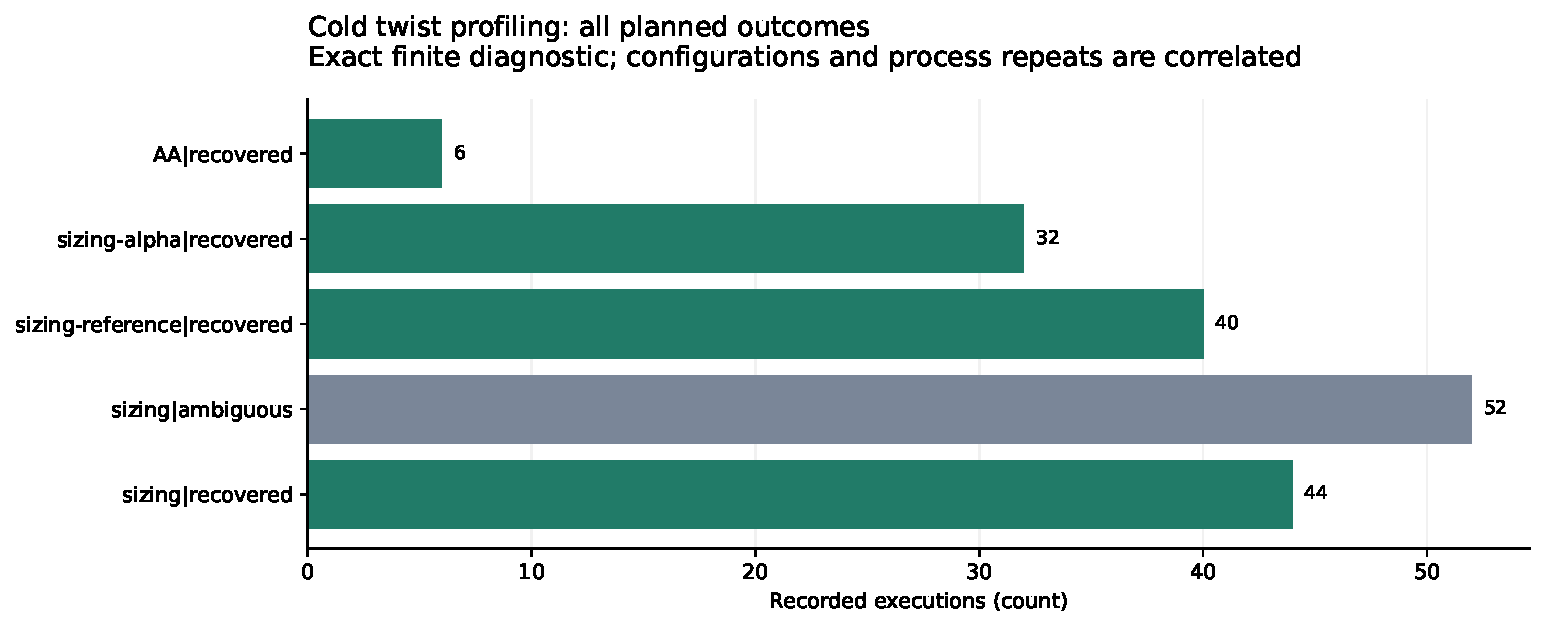
\includegraphics{OUTCOMES.pdf}
\caption{All recorded outcomes}
\end{figure}

\begin{figure}
\centering
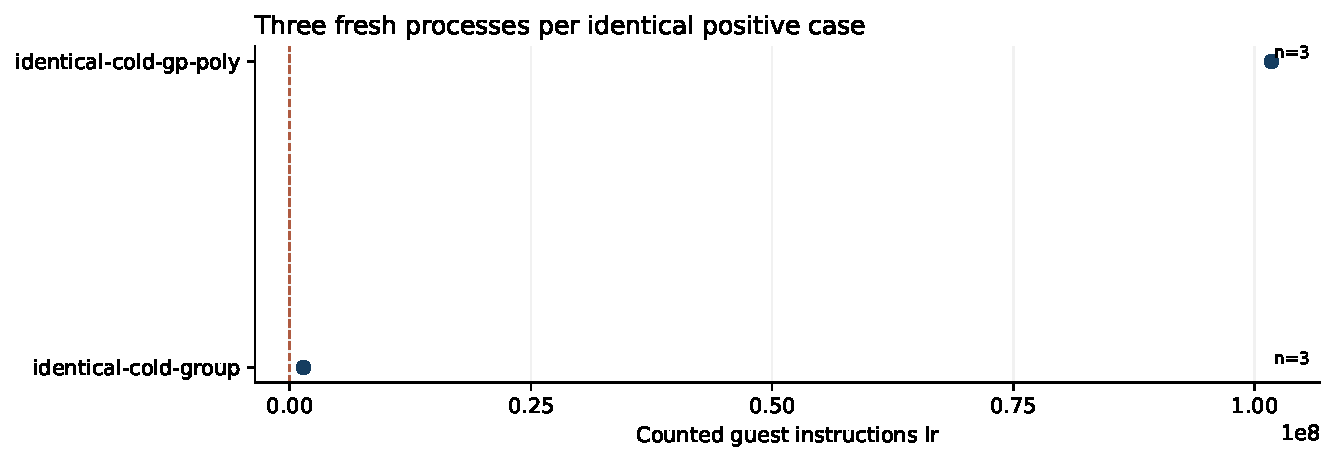
\includegraphics{AA.pdf}
\caption{A/A guest-instruction ranges}
\end{figure}

Sources: \href{../../execution-v16/PROTOCOL.md}{frozen protocol},
\href{../../execution-v16/analysis-v1/.artifacts.json}{native data
manifest}, \href{../../execution-v16/FROZEN.json}{source/byte pins}.
\href{../../execution-v16/audit-v1/ADMISSION.json}{Independent GP
admission}.

Reproduction and raw-object manifests are linked from the evidence
directory. The user-confirmed store is
\texttt{setec-astronomy-artifacts}, region us-east-2. No NIST,
asymptotic, novelty or calibrated-GAE result is established.

\end{document}
